\begin{frame}{recall: x86-64 general purpose registers}
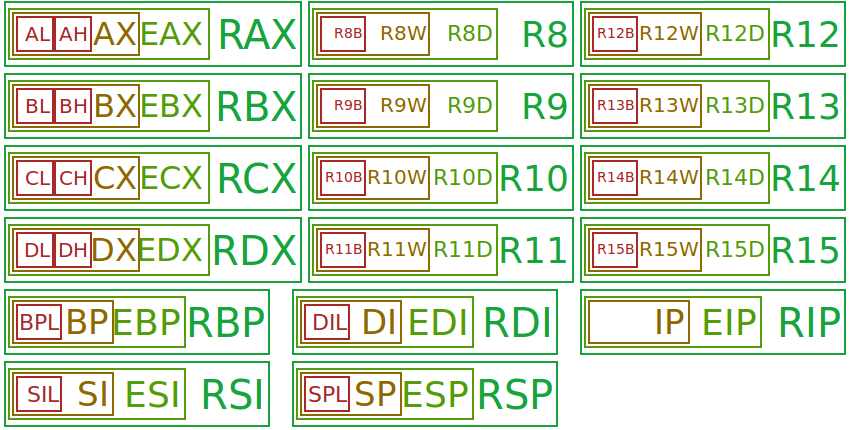
\includegraphics[width=\textwidth]{../asm/x86-gprs}
\imagecredit{Figure: Immae via Wikipedia}
\end{frame}

\begin{frame}[fragile,label=overlapEx]{overlapping registers (1)}
    \begin{itemize}
    \item setting 32-bit registers --- clears corresponding 64-bit register
\begin{asmcodeNL}
movq $0xFFFFFFFFFFFFFFFF, %rax
movl $0x1, %eax
\end{asmcodeNL}
        \item \%rax is {\tt 0x1} ({\small not {\tt 0xFFFFFFFF00000001}})
    \end{itemize}
\end{frame}
\begin{frame}[fragile,label=overlapEx2]{overlapping registers (2)}
\begin{itemize}
    \item setting 8/16-bit registers: don't clear 64-bit register
\begin{asmcodeNL}
movq $0xFFFFFFFFFFFFFFFF, %rax
movb $0x1, %al
\end{asmcodeNL}
    \item \%rax is {\tt 0xFFFFFFFFFFFFFF01}
\end{itemize}
\end{frame}

